\chapter{Aprendizaje automático}

En este capítulo se profundizará en el área de \emph{aprendizaje automático}
abarcando la representación de palabras y oraciones dadas por codificaciones del
tipo one-hot, word embeddings, conceptos de aprendizaje supervisado y no
supervisado, modelos de clasificación, ajuste de hiperparámetros, y métricas.

\section{Orígenes y evolución}

El aprendizaje automático es el campo de la inteligencia artificial que busca
desarrollar programas que aumáticamente mejoren en base a la experiencia. Estos
métodos difieren del típico paradigma de implementación donde en lugar de ser
``programado`` es ``entrenado``. Tal entrenamiento consiste en disponerle al
algoritmo información en forma de ejemplos con el fin de reconocer patrones
estadísticios y eventualmente determinar reglas que sirvan para automatizar una
tarea.

Por moderno que pueda parecer este campo, tuvo sus comienzos en los años 50 a
partir del famoso \emph{Test de Turing} que consistía de una máquina cuyo
objetivo era engañar a un humano haciéndole creer que se encontraba delante de
otra persona en lugar de un ordenador. Llegando a la conclusión de que los
computadores de propósito general, podrían ser capaces de aprender y ser de
alguna manera originales.
\footnote{\url{https://www.turing.org.uk/scrapbook/test.html}}

En los últimos años varias aplicaciones se han beneficiado de esta área, desde
programas relacionados con la detección fraudulenta de transacciones con tarjeta
de credito, sistemas de recomendación que guían usuarios en un servicio de
acuerdo a sus preferencias, o incluso vehículos que se manejan sin necesidad de
la intervención del conductor. Al mismo tiempo, una importante cantidad de
avances teóricos y algorítmicos se fueron realizando formando las bases de este
campo. TODO: Poner referencias a los ejemplos.

Aún con estos increibles logros, no se conoce aún como crear computadoras que
aprendan al nivel que las personas lo hacen. No obstante, se han desarrollado
algoritmos que se han aproximado a este objetivo siendo efectivos para varios
tipos de problemas.

\section{Aprendizaje supervisado}

El aprendizaje supervisado es una subárea del aprendizaje automático cuyo
objetivo es deducir una modelo a partir de datos anotados que permita mapear
ejemplos no vistos previamente. Esta información está compuesta por un conjunto
de ejemplares y sus correspondientes etiquetas, en ocasiones dada por un
anotador humano, la cual indica el resultado del modelo a partir del dato como
entrada. Las etiquetas pueden ser categóricas o continuas determinando un
problema de clasificación o regresión. Algunas tareas más frecuentes de
clasificación son la categorización de documentos, reconocimiento de lenguaje
ofensivo, o análisis de sentimiento. Mientras que para regresión, lo son las
estimaciones de precios de artículos, objetos, o viviendas.

El resultado de ejecutar un algoritmo de machine learning supervisado se puede
expresar como una función $f(\vect{x})$ que recibe un ejemplar $\vect{x}$ como
entrada y genera un vector $\vect{y}$ de salida codificado de la misma manera
que las etiquetas. Las muestras utilizadas para ajustar $f$ estan dadas por
vectores $\{\vect{x}_1, ..., \vect{x}_n\}$ y anotaciones $\{y_1, .. y_n\}$
conformando el \emph{conjunto de entrenamiento}.

La forma precisa de $f$ es determinada durante la fase de entrenamiento. Una vez
transcurrida, se puede estimar la identidad de nuevos datos etiquetados
pertenecientes al \emph{conjunto de test} con el fin de evaluar la performance
del modelo. En el caso que la predicción se aproxime a la esperada para estas
nuevas entradas, entonces el modelo habría logrado generalizar la tarea.

Sin embargo, los modelos de aprendizaje supervisado están limitados por la
disponibilidad de las anotaciones y la dificultad para obtenerlas.
Algunas tareas son relativamente sencillas para etiquetar para cualquier
persona, (e.g. como determinar si en una foto aparece un gato), mientras que en
otros puede llegar a requerir humanos que sean expertos de dominio (e.g.
abogados, médicos, lingüistas, etc).

\section{Aprendizaje no supervisado}

En contraste al método anterior, el aprendizaje no supervisado consiste en
descubrir automáticamente patrones sobre los datos de entrenamiento que permitan
explicarlos sin depender de datos de anotados. Es considerada como una parte del
área del análisis y exploración. Es por eso que no pueden ser evaluados
basándose en exactitud o precisión, si no más bien en la cantidad de información
que podamos extraer de los datos a partir del uso de estas técnicas. Algo a
considerar es la facilidad para disponer de estos datos (en comparación a los no
supervisados) al no requerir ningún tipo de supervición humana.

\section{Codificación de características}

Los modelos de aprendizaje automático dependen fuertemente de como se
representen los datos de entrada que uno tiene disponible. Preparar los
ejemplares para acoplarse apropiadamente a un algoritmo de machine learning con
el fin de mejorar la performance del modelo es una de las tareas las cuales los
científicos de datos disponen la mayor parte de su atención y tiempo. Alguna de
las obligaciones que incluye son la imputación de valores faltantes, manejo de
valores atípicos, estandarización y escalado, transformación de características
numéricas a categóricas, y codificación.

En particular pondremos nuestro foco en la codificación de características
desarrollando métodos del tipo \emph{one-hot} y \emph{word embeddings}.

\subsection{One-hot encoding}

A menudo los datos disponibles presentan características que no estan dadas en
un espacio continuo si no más bien categórico. Por ejemplo, se podría describir
el continente de un país por las clases \emph{inAsia}, \emph{inAfrica},
\emph{inEurope}, \emph{inSouthAmerica}, \emph{inNorthAmerica} siendo
eficientemente representables con enteros $[0, 1, 2, 3, 4]$. De esta manera, si
tenemos una serie de variables categóricas, estas pueden codificarse enumerando
por variable cada uno de sus objetos. Esta representación es conocida como
\emph{ordinal encoder}.

\begin{equation*}
    \begin{bmatrix}
         & inContinent\\
        Argentina & 3 \\
        Brasil & 3 \\
        España & 2 \\
        USA & 4  \\
        Italia & 2 
    \end{bmatrix}
\end{equation*}

Otra opción es usar un esquema \emph{one-of-K} que
transforma una característica categórica con $N$ clases, en $N$ categorias
binarias con una de ellas 1 y el resto 0. Para el ejemplo anterior tendríamos:

\begin{equation*}
\begin{bmatrix}
    & inAsia & inAfrica & inEurope & inSouthAmerica & inNorthAmerica \\
    Argentina & 0 & 0 & 0 & 1 & 0 \\
    Brasil & 0 & 1 & 0 & 1 & 0 \\
    España & 0 & 0 & 1 & 0 & 0 \\
    USA & 0 & 0 & 0 & 0 & 1 \\
    Italia & 0 & 0 & 1 & 0 & 0
\end{bmatrix}
\end{equation*}

La misma técnica es válida si se quisiera representar oraciones o documentos del
lenguaje natural. Supongamos que tenemos los documentos.

\begin{center}
    $D_1$: ``El sol es una estrella, no es un planeta.`` \\
    $D_2$: ``La tierra es un planeta.``    
\end{center}

Basado en  estos dos textos, un vocabulario de 9 palabras distintas es
construido. Por lo tanto cada documento es representado como un vector de 9
dimensiones.

\begin{equation*}
    \begin{bmatrix}
        & El & sol & es & una & estrella & no & un & planeta & tierra \\
        D_1 & 1 & 1 & 2 & 1 & 1 & 1 & 1 & 1 & 0  \\
        D_2 & 0 & 0 & 1 & 0 & 0 & 0 & 1 & 1 & 1 
    \end{bmatrix}
\end{equation*}

Observar que para este caso una codificación ordinal no sería adecuada dado que
se deberían enumerar todas las palabras del vocabulario.

Sin embargo, tomemos una oración dada en el contexto de planning (en particular
del dominio \emph{satellite} descripto en apéndice A). La siguiente secuencia
muestra un plan relajado de largo 4 asociado a una tarea STRIPS cuyos esquemas
de acción son $calibrate, switch\_on, take\_image,$ y $turn\_to$. El resto de
expresiones son objetos concretos del dominio. También es importante mencionar
que cada objeto de un cierto tipo está enumerado. Por ejemplo el objeto
$instrument1$ es del tipo $instrument$ cuyo índice es $1$. 

\begin{align*}
    & (calibrate\ satellite0\ instrument1\ groundstation0) \\
    & (switch\_on\ instrument1\ satellite0) \\
    & (take\_image\ satellite0\ planet5\ instrument1\ image1) \\
    & (turn\_to\ satellite0\ groundstation0\ planet5) \\
\end{align*}

La primera dificultad para codificarla surge bajo la pregunta de a que se
identifica como una palabra de la oración. Una primera iniciativa es definir una
acción como un token y utilizar un one hot encoding. No obstante, por lo general
una acción no suele ocurrir más de una vez en un plan de la tarea lo cual se
perdería la información de la frecuencia en que ocurren los objetos en la
secuencia. No solo es clave capturar los objetos si no también el índice del
cual se trata. Por lo tanto respetar su numeración es igual de relevante. Por
último cada acción debe mantener la misma cantidad de componentes en su
representación vectorial, independientemente del esquema o el número de
parámetros que reciba, y se debe asegurar el orden de la secuencia.

Para solventar estas dificultades se mantuvo un codificación one hot ordinal que
consiste en:

\begin{itemize}
    \item Cada elemento en la interfaz de una acción junto a su esquema son
    definidos como tokens. Eso incluye la numeración de los objetos.
    \item Cada vector que representa a una acción tiene dimensión $2 \times N +
    1$ siendo $N$ la longitud de la interfaz más larga de un esquema. Aquellas
    acciones con una interfaz más chica se les agrega un margen de $0's$ hasta
    completar el largo requerido.
    \item Los esquemas de acción son enumerados en el rango $1, ..., M$ con $M$
    la cantidad de esquemas.
    \item El tipo de los objetos son enumerados en el rango de $1, ..., K$. con
    $K$ la cantidad de tipos.
    \item Si un objeto tiene el índice $i$ se lo incrementa en 1 (para evitar que
    aquellos objetos que empiecen con indice 0 se malinterpreten como margenes).
\end{itemize}

Por ejemplo si la enumeración de las esquemas y tipos fuesen los siguientes:

\begin{align*}
    &\{calibrate: 1,\ turn\_to: 2,\ switch\_on:3,\ take\_image:4 \} \\
    &\{satellite: 1,\ instrument: 2,\ planet: 3,\ groundstation: 4,\ image: 5\}
\end{align*}

En este la longitud de la interfaz más larga es 4, entonces cada acción tendrá
asociado un vector de dimensión $2 \times 4 + 1 = 9$ y la codificación
resultante sería:

\begin{align*}
    (calibrate\ satellite0\ instrument1\ groundstation0) &: (1\ 1\ 1\ 2\ 2\ 4\ 1\ 0\ 0) \\
    (switch\_on\ instrument1\ satellite0) &: (3\ 2\ 2\ 1\ 1\ 0\ 0\ 0\ 0) \\
    (take\_image\ satellite0\ planet5\ instrument1\ image1) &: (4\ 1\ 1\ 3\ 6\ 2\ 2\ 5\ 2) \\
    (turn\_to\ satellite0\ groundstation0\ planet5) &: (2\ 1\ 1\ 4\ 1\ 3\ 6\ 0\ 0) \\
\end{align*}

\subsection{Vectores de palabras (Word embeddings)}

Un vector denso de palabras (comúnmente conocido como word embedding, en inglés)
es una de las técnicas de representación de vocabulario más popular en el área
del procesamiento de lenguaje natural.

Si bien hay distintas formas de representar palabras en una serie de documentos,
los word embeddings proveen otra perspectiva que busca encontrar una
representación vectorial compacta donde cada dimensión logre capturar las
propiedades subyacentes y latentes de la palabra (sintácticas o semánticas). De
esta manera, los embeddings son superiores a una representación que permanece en
un nivel poco profundo.

Su principal característica  es que las palabras relacionadas entre sı́ (ya sea
por contexto, semántica o sintaxis) se encuentren cercanas en el espacio
vectorial al cual se proyectan. Por ejemplo, si tenemos las oraciones: ``Que
tengas una buena mañana`` y ``Que tengas una buena tarde``. Difieren
semánticamente solo por las palabras ``mañana`` y ``tarde``. No obstante, se
utilizan en contextos similares, lo cual esperariamos que esten cercanos
vectorialmente.

Otro ejemplo muy famoso que deja en evidencia el concepto de \emph{analogía} en
word embeddings, es el que se muestra en la figura 3.1. En ella se identifican
por medio de barras de colores la dimensión de los vectores asociados a las
palabras \emph{king}, \emph{man}, \emph{woman}, \emph{queen}, y la operación
vectorial \emph{king - man + woman}. Cada dimensión se encuentra en la escala de
$[-2, 2]$ y se le asigna el color de rojo para valores cercanos al extremo
derecho, azúl para las del extremo izquierdo, y blanco para las que se
encuentren alrededor del 0.  Algo a notar es que \emph{man} y \emph{woman} son
mucho más similares de lo que cada uno es con \emph{king} o \emph{queen}. No
obstante, las franjas roja y azúl que se muestran para cada uno de los ejemplos
indicando que son parecidos en tal dimensión. Probablemente corresponda a alguna
característica humana aunque se desconoce que puedan llegar a significar
debido a la poca interpretabilidad del espacio al cual se proyecta. 

Aun así, lo importante es la comparación entre palabras. Dado que ahora tienen
una representación vectorial, se pueden sumar o restar obteniendo nuevos
resultados que forman parte del espacio. Este es el caso del vector dado por
\emph{king - man + woman}. No conocemos que dimensiones exactamente capturan que
rey es utilizado para identificar al monarca de un reino, pero se puede
substraer el caracter masculino del vector \emph{man} y agregar las de
\emph{woman} esperando que se aproximen a las de \emph{queen}.
Sorprendentemente, de un total de 400000 palabras sobre las cuales se realizó el
experimento, reina fue la palabra más cercana. Los detalles del mismo se pueden
ver desde \footnote{\url{https://jalammar.github.io/illustrated-word2vec/}}.

\begin{figure}
    \centering
    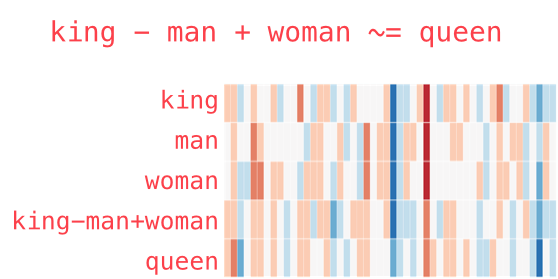
\includegraphics[scale=0.68]{figures/king-analogy-viz.png}
    \caption{Vectores de palabras para ``king``, ``man``, y ``woman``}
\end{figure}


\subsubsection{Modelos de lenguaje}

Después de ver el potencial de los embeddings, surge la pregunta, ¿cómo
funcionan internamente? ¿de qué manera se obtienen estos vectores de palabras?
Para ello debemos acudir al concepto de modelos de lenguaje neuronales.

Los embeddings de palabras obtienen su representación a partir de otras sobre
las que co-ocurren \citep{} y se obtienen a partir del texto que queremos
representar. Para ello se hace uso de muchos documentos no supervisados y luego
se representa la compañia de una palabra a partir de una ventana alrededor de
ella que la contiene. Moviendo la ventana a lo largo de todo el documento, se
generan ejemplares de entrenamiento para realizar una tarea de \emph{pretexto}.

Los tipos de tareas de pretexto que mencionaremos son \emph{contionous bag of words} y \emph{skipgram}

\subsubsection{Skipgram}

Es un método desarrollado en \citep{Mikolov-2013} que consiste de una red
neuronal cuyo objetivo de entrenamiento es encontrar representaciones de
palabras que sean útiles para predecir una palabra dado su contexto. Por ejemplo
la oración ``Que tengas una buena tarde`` y un contexto de tamaño 3,
obtendriamos las secuencias ``Que tengas una``, ``tengas una buena``, y ``una
buena tarde``. A cada ventana removemos el caracter del medio, ``Que \_\_ una``,
``tengas \_\_ buena``, ``una \_\_ tarde``. Finalmente, en base a los restantes
intentamos predecir aquel que se quitó. Para esta simple oración se podrían
construir 3 ejemplares:

\begin{equation*}
    \begin{bmatrix}
        Input_1 & Input_2 & Target\\
        Que & una & tengas  \\
        tengas & buena & una \\
        una & tarde & buena
    \end{bmatrix}
\end{equation*}

Una vez repetido esto para todas las oraciones del conjunto de datos con el
que se está trabajando, se asigna una representación inicial aleatoria
a las palabras. Estas se iran actualizando a medida que la red neuronal
entrene para la tarea de predicción. El resultado final del modelo neuronal
es, para cada palabra en el vocabulario, la probabilidad de que sea la faltante.

Más formalmente, dada una secuencia de palabras $w_1, w_2, w_3, ... w_T$,
maximizar la probabilidad media de registro:

\begin{align*}
    \frac{1}{T} \sum_{n=1}^{T} 
                    \sum_{-c \leq j \leq c} \log p(w_{t+j} | w_t)
\end{align*}

donde $c$ es la ventana de contexto. En la formulación básica de skipgrams el
valor de $p(w_{t+j}|w_{t})$ está definido como una función de softmax:

\begin{align*}
    p(w_{t+j}|w_{t}) = \frac{e^{v'_{w_O} v_{w_I}}}{\sum_{w=1}^{W} e^{v'_{w} v_{w_I}}}
\end{align*}

donde $v_w$ y $v'_w$ son las proyecciones vectoriales de entrada y salida de $w$
y $W$ es el número de palabras en el vocabulario.

\subsubsection{Continous bag of words}

\subsubsection{Representación vectorial de oraciones}

En \citep{Iacobacci-2016} se explican como utilizar word embeddings para
desambiguación de sentidos, proponiendo distintos métodos de codificación de
instancias de entrenamiento a partir de un modelo de lenguaje, con el fin
de incluirlos en una arquitectura supervisada. En particular, detallaremos
algunos métodos más sencillos y que son común en la literatura para resolver
tareas de clasificación que involucren la manipulación de texto.

\textbf{Concatenación}. Este método consiste en concatenar los vectores de las
palabras que conforman la oración a codificar obteniendo un vector de largo
igual a la suma de las dimensiones de los vectores individuales. En este caso,
el problema evidente que surge es la representación de oraciones con distinto
largo y el tamaño del vector resultante.

\textbf{Promedio}. Como su nombre lo indica, este método computa el centroide de
los embeddings de todas las palabras que conforman una oración. Usualmente esta
codificación resulta ser adecuada siempre y cuando los vectores de las palabras
se encuentren en la misma escala, lo cual no siempre suele ser el caso. Otro
problema menos evidente es la posibilidad de ocurrencia de palabras poco
representativas pero que tengan mucho peso en la suma, ignorando las ocurrencias
que nos interesan para la tarea que se intenta resolver.

\textbf{Promedio normalizado}. Por último, una mejora de la representación
anterior es la normalización por norma L2 de cada vector previo a realizar el
promedio.

\subsubsection{Word2Vec}

En \citep{Mikolov-Ilya-Kai-Greg-Jeffrey-2013} se presentaron dos arquitecturas
para calcular representaciones vectoriales continuas de palabras a partir de
conjuntos de datos muy grandes. El modelo de \emph{skip-grams continuos} y el de
\emph{bolsa de palabras continuos} (CBOW)

El modelo de CBOW consiste en una red neuronal con una capa oculta lineal
donde todas las

Estos métodos utilizan redes neuronales para crear un modelo de lenguaje a
partir de una tarea de pretexto. 

\section{Entrenamiento y evaluación}

\subsection{Validación cruzada}

\subsection{Búsqueda de hiperparámetros}

\section{Algoritmos de clasificación}

\subsection{Regresión logistica}

\subsection{XGBoost}

\subsection{Redes neuronales}

\section{Métricas de clasificación}